%%%%%%%% ICML 2020 EXAMPLE LATEX SUBMISSION FILE %%%%%%%%%%%%%%%%%

\documentclass{article}
\usepackage{times}
\usepackage{epsfig}
\usepackage{graphicx}
\usepackage{amsmath}
\usepackage{amssymb}
\usepackage{times}
\usepackage{epsfig}
\usepackage{graphicx}
\usepackage{amsmath}
\usepackage{amssymb}
% Include other packages here, before hyperref.
\usepackage{xcolor}
\usepackage[ruled,vlined,onelanguage]{algorithm2e}
\usepackage{setspace}
\usepackage{collcell}
\usepackage{xr}
\usepackage{natbib}
\usepackage{multirow}
\usepackage{subcaption}
\usepackage{mathtools}
\usepackage{colortbl,dcolumn}
\usepackage{algorithm2e}

% Include other packages here, before hyperref.

% If you comment hyperref and then uncomment it, you should delete
% egpaper.aux before re-running latex.  (Or just hit 'q' on the first latex
% run, let it finish, and you should be clear).
\usepackage[pagebackref=true,breaklinks=true,letterpaper=true,colorlinks,bookmarks=false]{hyperref}

% \cvprfinalcopy % *** Uncomment this line for the final submission

\def\cvprPaperID{****} % *** Enter the CVPR Paper ID here
\def\httilde{\mbox{\tt\raisebox{-.5ex}{\symbol{126}}}}

\newcommand{\todo}[1]{{\color{blue}TODO #1}}
\newcommand{\toref}[1]{{\color{red}REF #1 }}
\newcommand{\registered}{\textsuperscript{\tiny\textregistered}}
%\newcommand{\etal}{\textit{et al.}}
\renewcommand{\eqref}[1]{\hyperref[#1]{Eq.\ \ref*{#1}}}
\newcommand{\figref}[1]{\hyperref[#1]{Fig.\ \ref*{#1}}}
\newcommand{\tabref}[1]{\hyperref[#1]{Table\ \ref*{#1}}}
\newcommand{\secref}[1]{\hyperref[#1]{Section\ \ref*{#1}}}
\newcommand{\algoref}[1]{\hyperref[#1]{Algorithm\ \ref*{#1}}}
\newcolumntype{C}[1]{>{\centering}m{#1}}
\newcommand{\N}{{\cal N}}
\newcommand{\std}[1]{ \normalfont \color{darkgray}\footnotesize{$\pm$#1} }

% SYMBOL
\newcommand{\E}{{\mathbb E}}

\hypersetup{
    colorlinks=true,
    linkcolor=blue,
    filecolor=magenta,      
    urlcolor=blue,
}

\urlstyle{same}

% Recommended, but optional, packages for figures and better typesetting:
\usepackage{microtype}
\usepackage{booktabs} % for professional tables

% hyperref makes hyperlinks in the resulting PDF.
% If your build breaks (sometimes temporarily if a hyperlink spans a page)
% please comment out the following usepackage line and replace
% \usepackage{icml2020} with \usepackage[nohyperref]{icml2020} above.
\usepackage{hyperref}

% Attempt to make hyperref and algorithmic work together better:
\newcommand{\theHalgorithm}{\arabic{algorithm}}

% Use the following line for the initial blind version submitted for review:
%\usepackage{icml2020}

% If accepted, instead use the following line for the camera-ready submission:
\usepackage[accepted]{icml2020}

% The \icmltitle you define below is probably too long as a header.
% Therefore, a short form for the running title is supplied here:
\icmltitlerunning{Bayesian active learning for production. Supplementary Material}

\begin{document}

\twocolumn[
\icmltitle{Supplementary Material}]

\section{Implementation details}
Our methodology is as follows. We train a VGG-16 \citep{zhang2015accelerating} pretrained on ImageNet~\citep{imagenet_cvpr09}. Our initial training set contains 500 samples. We estimate the uncertainty using 20 MC samples and label the 100 most uncertain elements. Following \citet{gal2017deep}, we reset the weights to their initial value between steps. 

\section{Imbalanced datasets}
 
How to deal with imbalanced datasets is an entire area of research \citep{krawczyk2016learning}, but little has been done to deal with it when we are not aware of the \textit{a priori} class distribution. In consequence, the active learning model may quickly overfit to the more popular classes and reduce the effectiveness of active learning procedure. From \citet{gal2017deep}, it is known that Bayesian active learning will favor underrepresented classes. But, we find the reported experiments to be too simple. We  test this hypothesis in a controlled environment where we can set the number of unrepresented classes. 

In \tabref{fig:imbalanced}, we took the standard CIFAR100 dataset and we mimic an imbalanced dataset where few classes have a high number of examples. A class selected to be underrepresented sees its number of samples to be reduced by 75\%. When we increase the number of underrepresented classes, the gain of using MC-Dropout versus random sampling becomes more obvious. This is due to regions on the learned manifold associated with underrepresented classes to be highly uncertain. In consequence, these regions will be selected for labelling very early in the process.

% In this section, we investigated how common issues in deep learning are affecting active learning. While BALD is robust to data imbalance, it is highly affected by the annotation error or being under fitted.


\begin{table}
    \centering
    \begin{tabular}{llll}
    
    \toprule
    Dataset size &         5000 &        10000 &        20000 \\
    
    \hline
   $\Delta =10$ \\
    BALD &  4.39 \std{0.4} &  3.99 \std{0.01} &  3.57 \std{0.05} \\
    Entropy &  4.71 \std{0.02} &  4.54 \std{0.07} &  3.94 \std{0.01} \\
    Random &  4.52 \std{0.09} &  4.10 \std{0.03} &  3.71 \std{0.05} \\
    \hline
   $\Delta =25$ \\
    BALD &  4.40 \std{0.03}	&4.04\std{0.03} &	3.61\std{0.08} \\
    Entropy &  4.76 \std{0.02} &  4.68 \std{0.08} &   4.00 \std{0.01} \\
    Random &  4.58 \std{0.08} &  4.18 \std{0.04} &  3.75 \std{0.01} \\
    \hline 
   $\Delta =50$ \\
    BALD &  4.49 \std{0.08} &   4.07 \std{0.02} &   3.66 \std{0.04} \\
    Entropy &  4.83 \std{0.04} &  4.60 \std{0.14} &  4.07 \std{0.28} \\
    Random &  4.62 \std{0.03} &   4.21 \std{0.02} &   3.76 \std{0.04} \\
    \end{tabular}
    \caption{Effect of using active learning on imbalanced versions of CIFAR100. $\Delta$ is the number of class that contains 25\% of their data. From \citep{gal2017deep}, we know that BALD is robust to imbalanced datasets, but the study was not extensive. While BALD is robust to imbalanced datasets, the effect is catastrophic when using Entropy.  Performance averaged over 5 runs.}
    \label{fig:imbalanced}
\end{table}

\section{Effect of convergence}

In \figref{fig:active_gain}, we computed the difference in performance between BALD and random. We call this measure the \textit{Active gain} $= NLL_{Random} - NLL_{BALD}$. When using an underfitted model, the gain goes negative i.e. you would be better to use random selection.

\begin{figure}
    \centering
    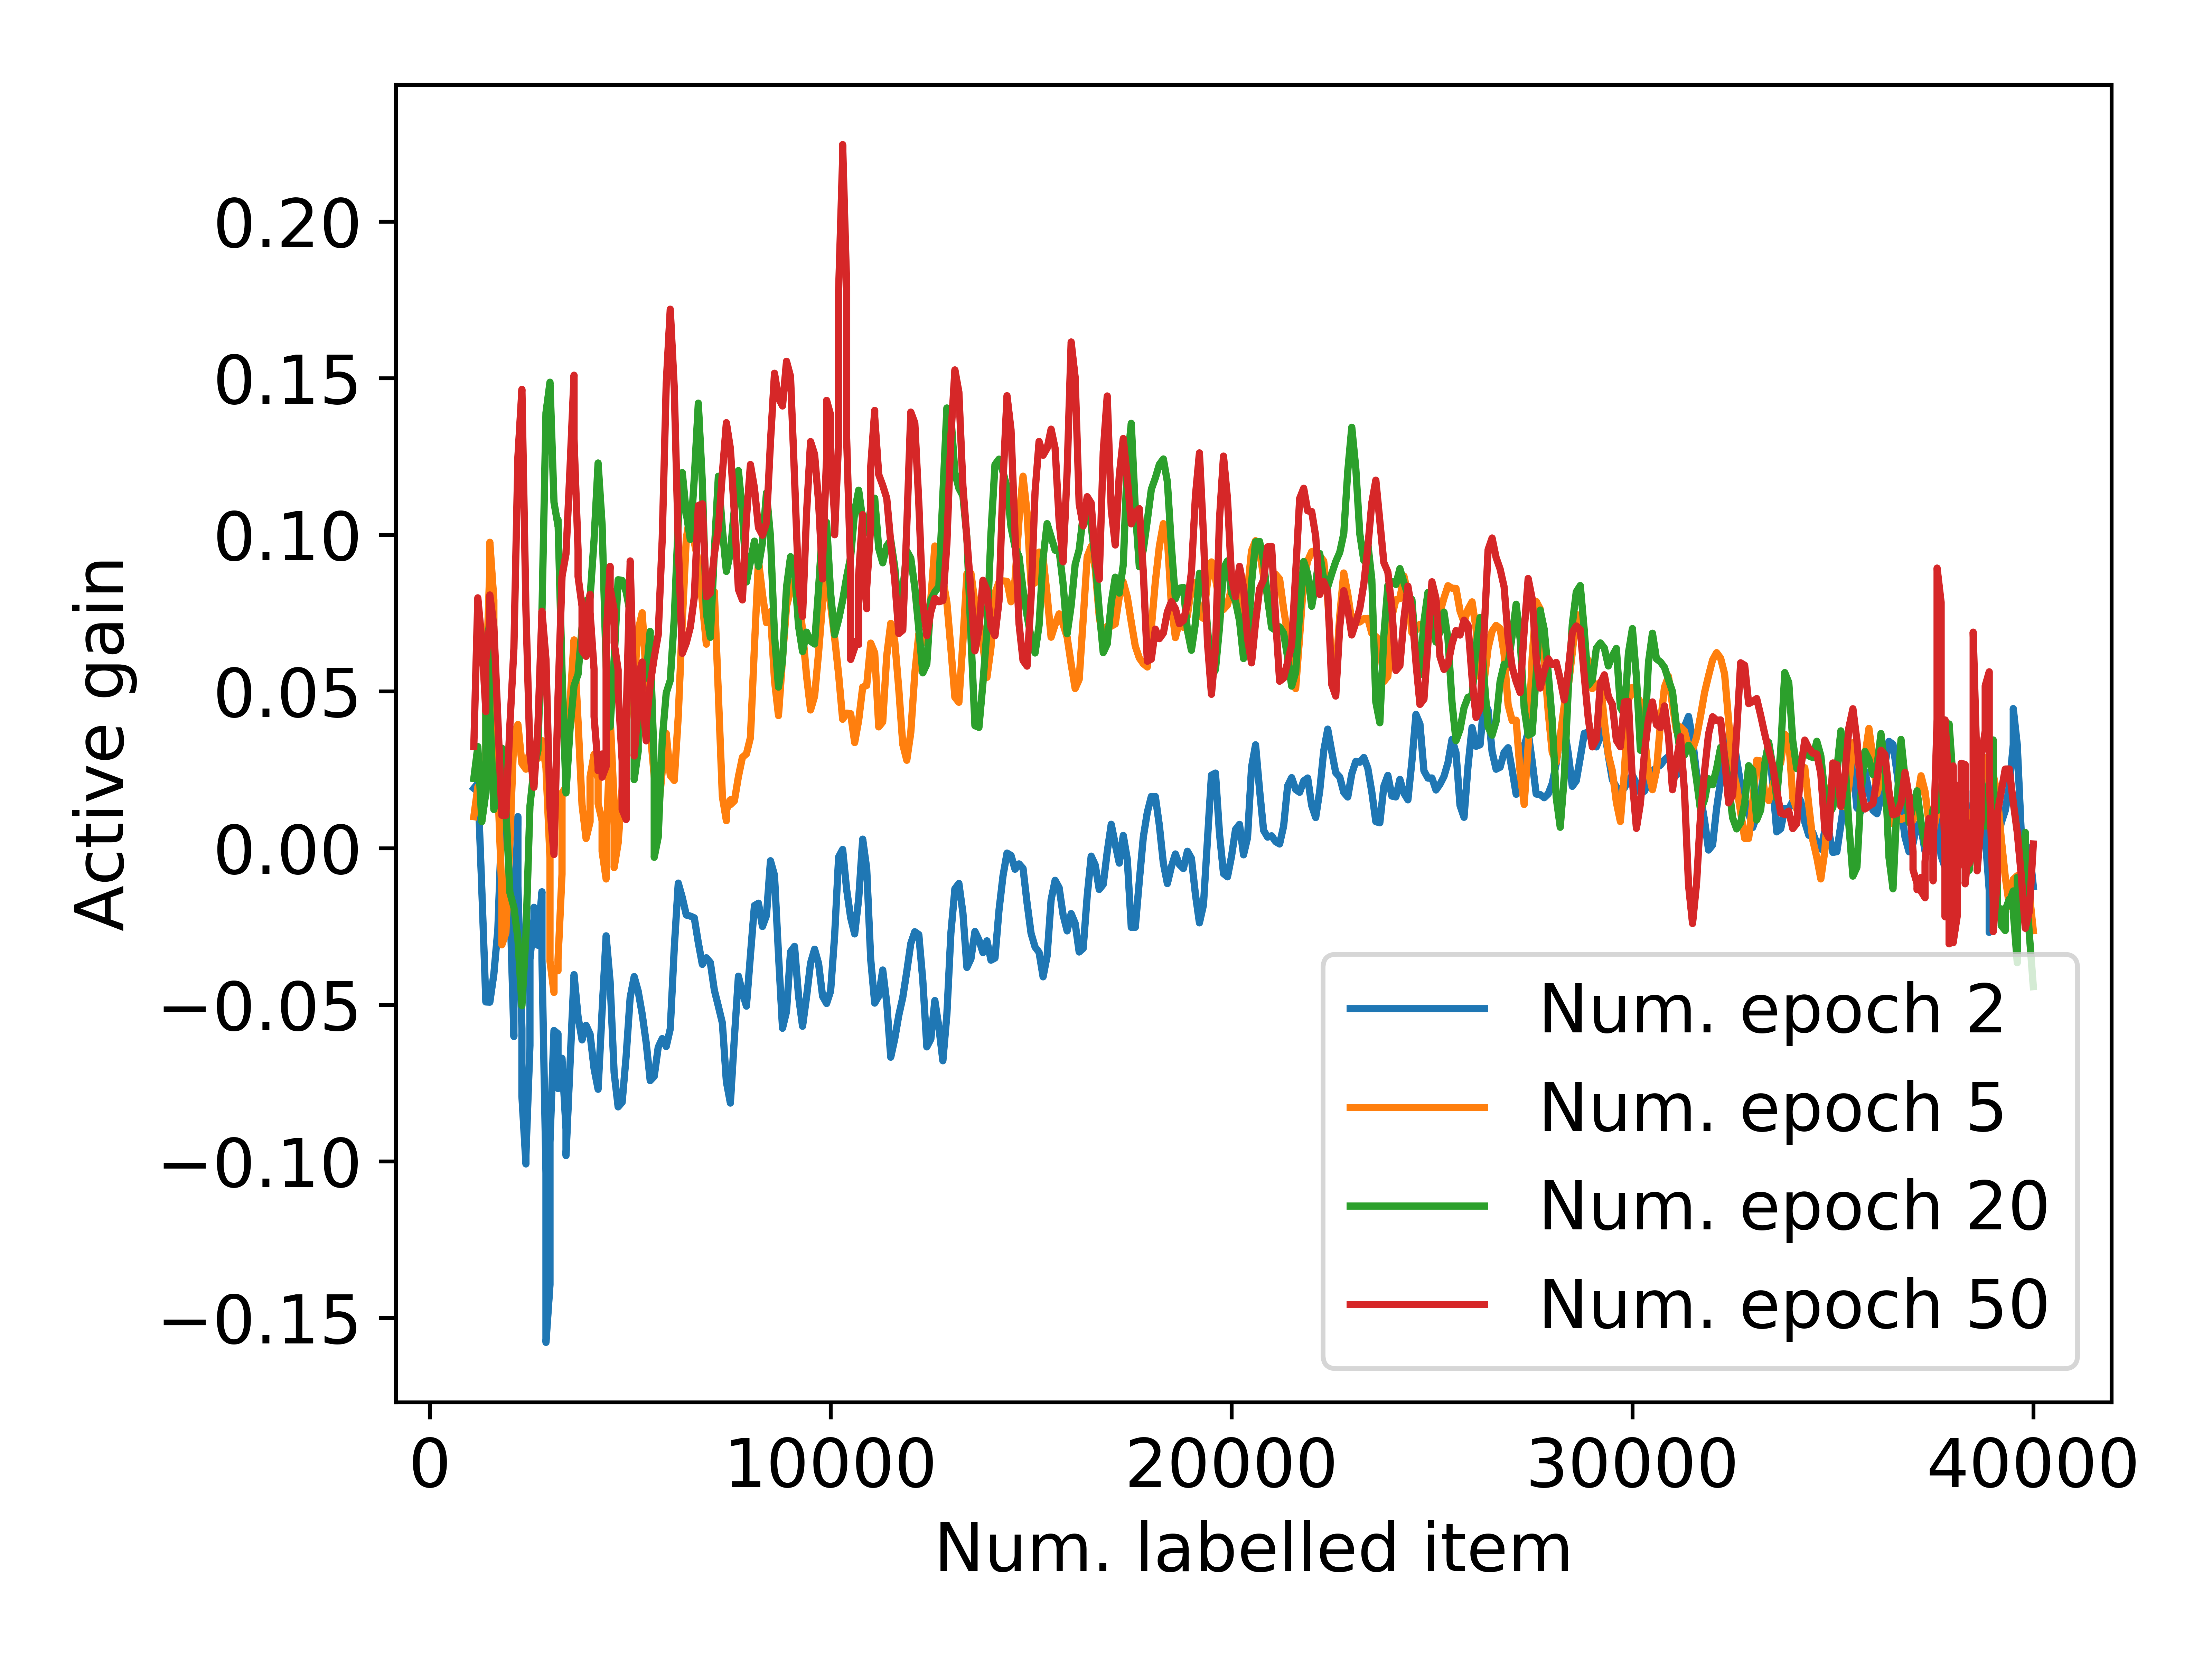
\includegraphics[width=0.5\textwidth]{fig/active_gain.png}
    \caption{Gain of using active learning when varying the number of training epochs. An underfitted model will cause harm to the model training and in this case, just using random would've been better.}
    \label{fig:active_gain}
\end{figure}

\section{Effect of reducing the pool size}
As part of the experiments, we test whether limiting the pool size would affect the performance of active learning. Our experiments in  \figref{fig:pool_size} show that whether to calculate the uncertainty for the whole pool data or a randomly selected subset, the performance of active learning is not affected. This leads to an the interesting outcome of limiting the uncertainty calculations (which is the most expensive part of an active learning loop) in production setup for faster active learning loops.

\begin{figure}
    \centering
    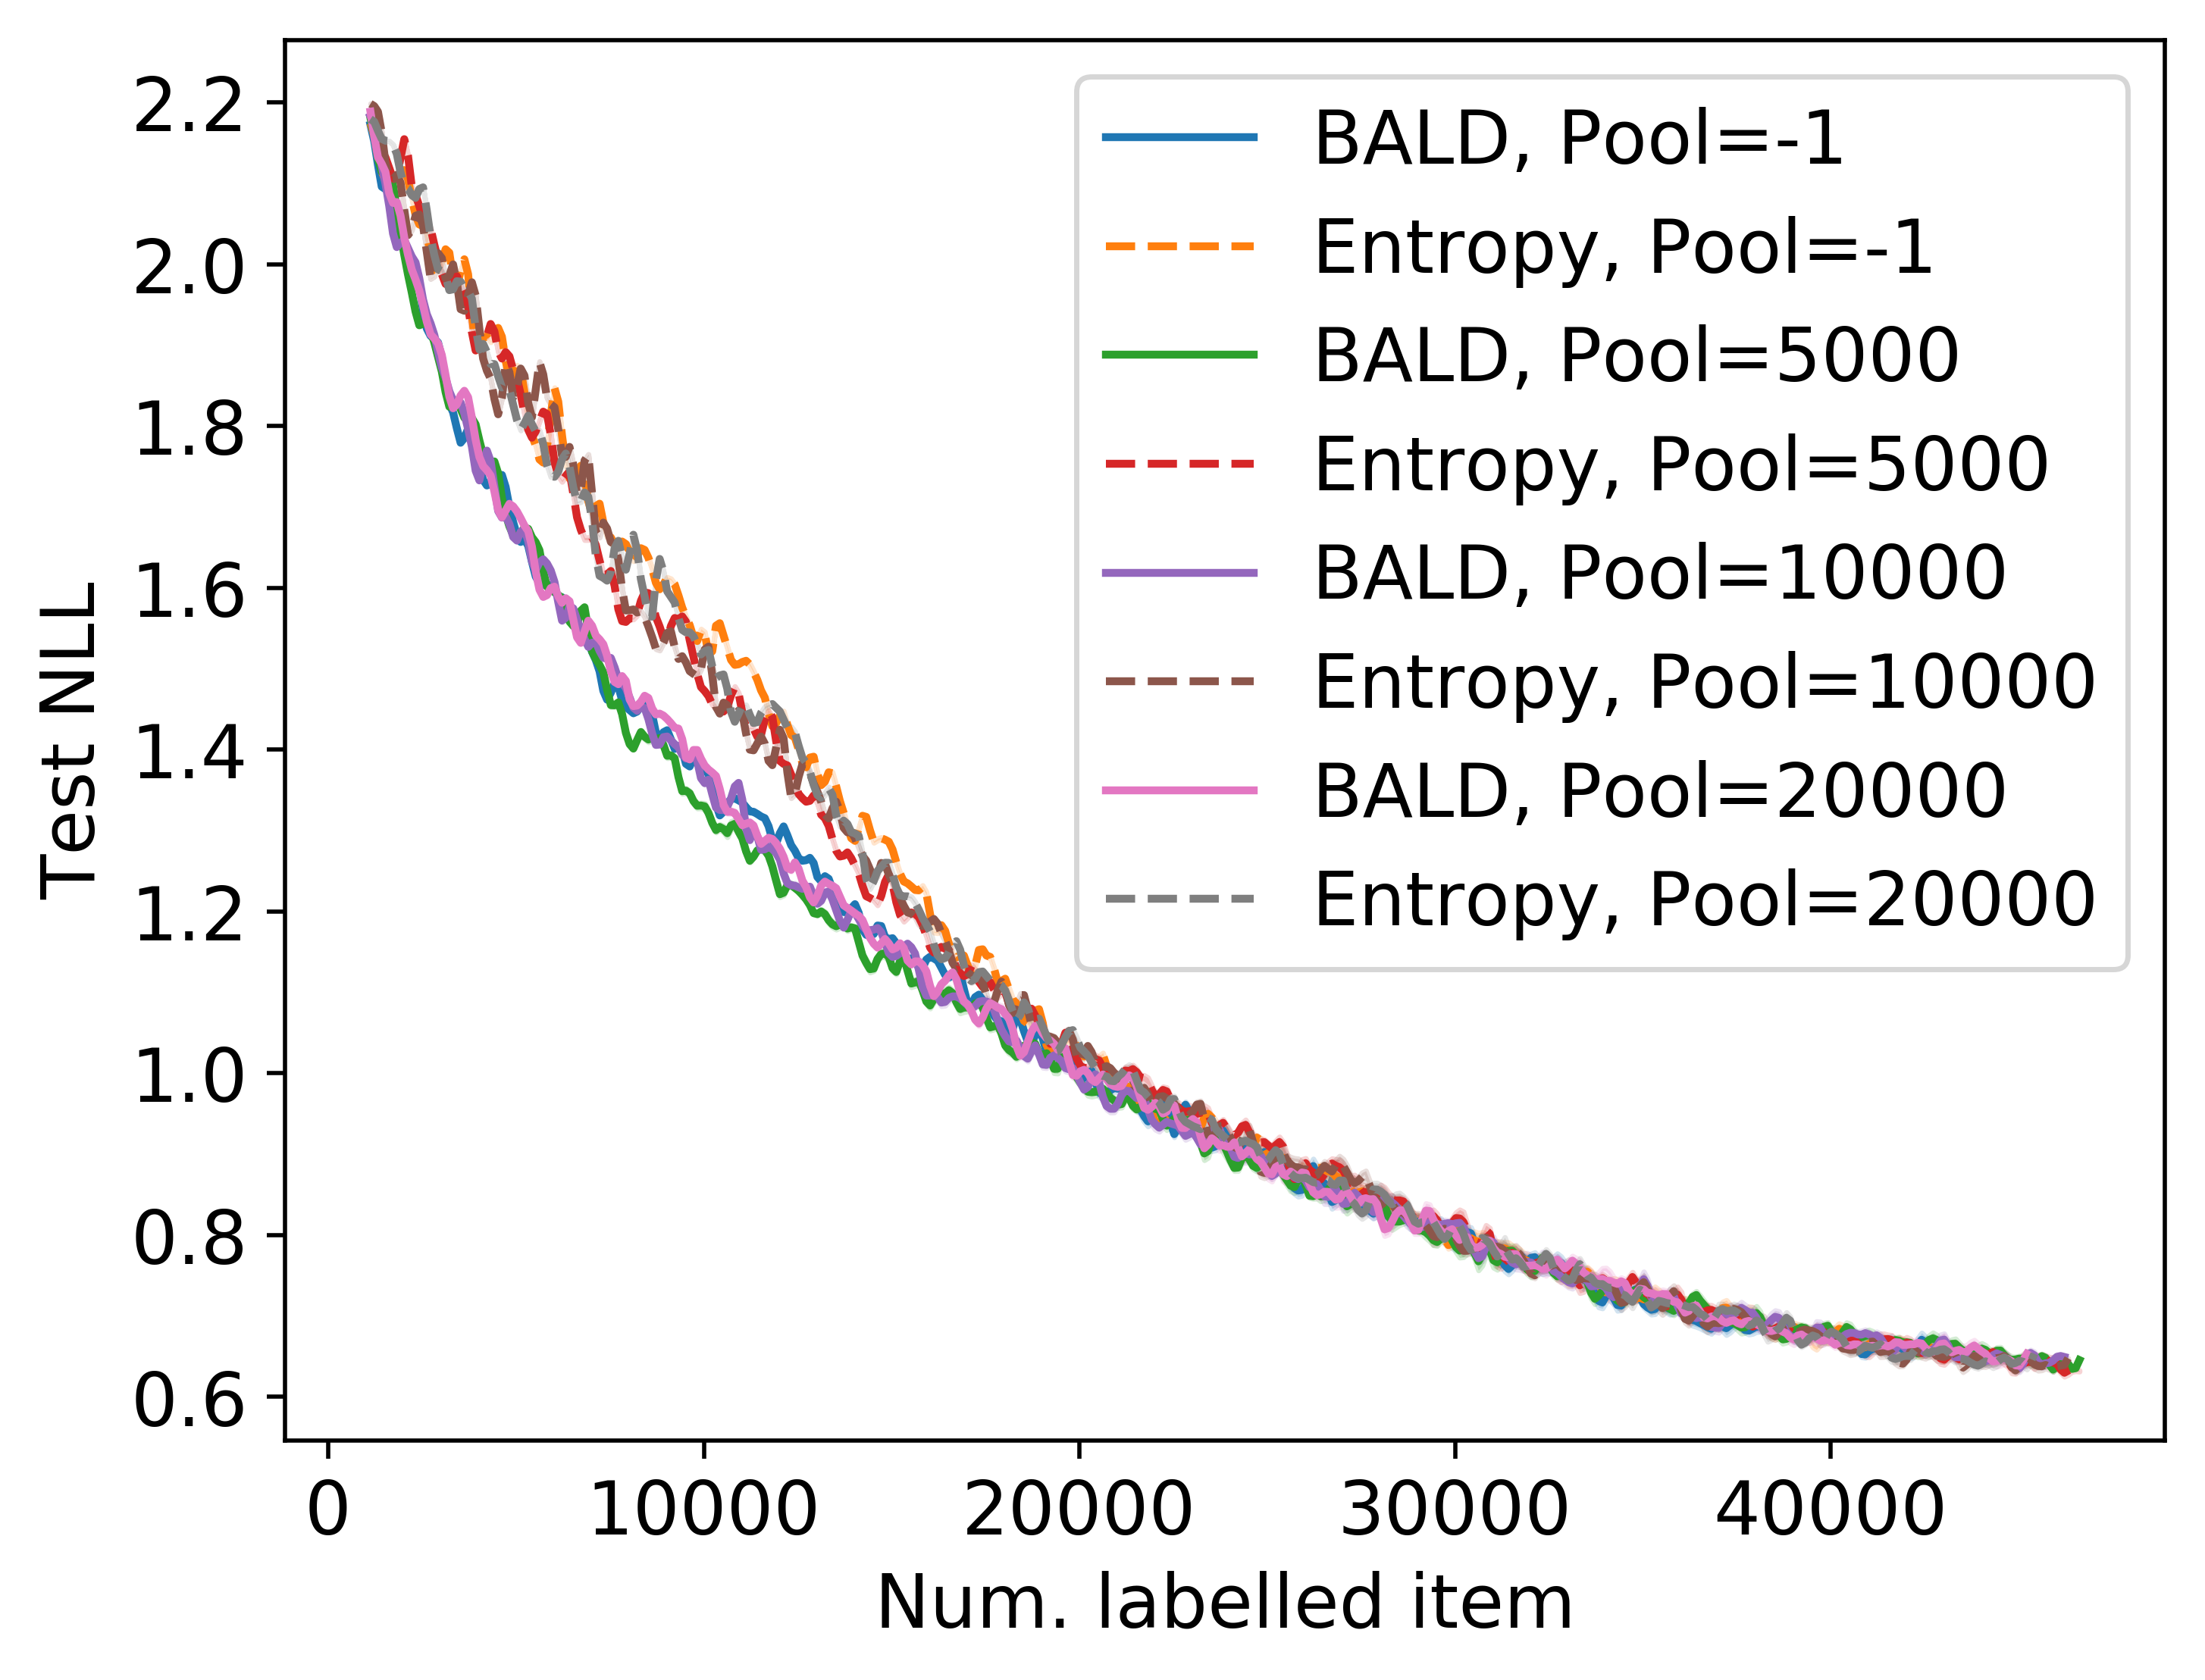
\includegraphics[width=0.4\textwidth]{fig/pol_size.png}
    \caption{Effect of reducing the size of the pool on CIFAR100. \textbf{-1} indicates no reduction. For all heuristics, the performance is not affected by the size of the pool showing that AL can be efficient when tuned properly.  Performance averaged over 5 runs.}
    \label{fig:pool_size}
\end{figure}

\begin{figure}
    \centering
    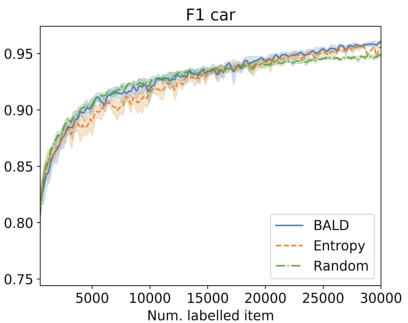
\includegraphics{fig/F1_Mio_tcd_annex.pdf}
    \caption{\textbf{F1 for the class \textit{car}}. BALD is great for underrepresented classes while not affecting more popular classes. Entropy decreases the performance on this class.}
    \label{fig:miotcd}
\end{figure}


\section{Bayesian active learning Library (BaaL)}

All the experiments in this paper have done using our publicly available Bayesian active learning library.  The goal of this library is to provide an easy to use but complete setup to test active learning on any project with few lines of code. We included features that current active learning libraries do not support. In particular, Bayesian methods such as MC-Dropout or Coresets are not widely available and there is no standard implementation of the active learning loop. Furthermore, research codebases are often hard to read and hard to maintain. Our proposed unified API could satisfy both research and industrial users.

 Our recently published open-source package named BaaL, aims at accelerating the transition from research to production. The core philosophy behind our library is to provide researchers with a well-designed API so that they focus on their novel idea and not on technical details. Our library proposes a task-agnostic system where one can mix-and-match any set of acquisition functions and uncertainty estimation methods.
The library consists of three main components:
\begin{enumerate}
    \item Dataset management to keep track and manage the labelled data $D_L$ and the unlabelled data $D_U$.
    \item Bayesian Methods i.e. MC-Dropout, MC-DropConnect and so on.
    \item Acquisition functions i.e. BALD, BatchBALD, Entropy and more.
\end{enumerate}

We provide full support for Pytorch \cite{paszke2017automatic} deep learning modules but our acquisition functions which are the most important part of active learning is implemented in  Numpy\cite{oliphant2006guide} and hence can be used on any platform. Our Data management module keeps track of what is labelled and what is unlabelled. We also provide facilitator methods to label a data point, update the pool of unlabelled data, and to randomly label a portion of the dataset. In our Bayesian module, we provide utilities to make any Pytorch model Bayesian with a single instruction. We also provide training, testing, and active learning loops that facilitate the active training procedure. Our acquisition functions are up-to-date with state-of-the-art methods. We provide easy to follow tutorials (https://baal.readthedocs.io/en/latest/) for each section of the library so that the user understands how each component works. Finally, our library is a member of Pytorch Ecosystem, which is reserved for libraries with outstanding documentation.

Our road-map has been indicated in the repository. Our current focus will include model calibration and semi-supervised learning. As more researchers contribute their methods to our library, we aim to become the standard Bayesian active learning library.

\end{document}